% !TEX program = lualatex
% !TEX encoding = UTF-8 Unicode
% !TEX spellcheck = de_DE
% 
% Vorlage für Bachelorarbeiten
% 
% Um die Vorlage mit LaTeX zu erstellen sind folgende Programme aufzurufen:
% > lualatex hauptdatei.tex
% > biber hauptdatei
% > lualatex hauptdatei.tex

\documentclass{scrbook}


\usepackage{tikz}

\usepackage{array,makecell}
\usepackage{caption}


\usepackage{tabularx}
    \renewcommand\tabularxcolumn[1]{m{#1}}
    \newcolumntype{C}{>{\centering\arraybackslash}X}

\newcommand{\ExternalLink}{%
    \tikz[x=1.2ex, y=1.2ex, baseline=-0.05ex]{% 
        \begin{scope}[x=1ex, y=1ex]
            \clip (-0.1,-0.1) 
                --++ (-0, 1.2) 
                --++ (0.6, 0) 
                --++ (0, -0.6) 
                --++ (0.6, 0) 
                --++ (0, -1);
            \path[draw, 
                line width = 0.5, 
                rounded corners=0.5] 
                (0,0) rectangle (1,1);
        \end{scope}
        \path[draw, line width = 0.5] (0.5, 0.5) 
            -- (1, 1);
        \path[draw, line width = 0.5] (0.6, 1) 
            -- (1, 1) -- (1, 0.6);
        }
    }


\usepackage{booktabs, caption, makecell}
\renewcommand\theadfont{\bfseries}
\usepackage{threeparttable}



%% Alle wichtigen Einstellungen sind in der Datei einstellungen.tex getätigt
%% und können dort verändert werden.
% !TEX root = hauptdatei.tex
% !TEX encoding = UTF-8 Unicode
% !TEX spellcheck = de_DE
%
% für mehr Informationen zu einzelnen Paketen siehe zum Beispiel:
% http://texdoc.org/pkg/paketname
% http://ctan.org/pkg/paketname


%% Setzen von Dokumentenoptionen:
%% (aquivalent zu \documentclass[<Optionen>]{...}

%%% Layout-Einstellungen
	\KOMAoptions{ 				% aquivalent zu \documentclass[<Optionen>]{...}
		fontsize=12pt,			% Standartschriftgröße
		bibliography=totoc,	% Bibliografie soll im Inhaltsverzeichnis auftauchen
		headings=normal,		% Größe und Abstand von Überschriften
		toc=listof,				% Verzeichnisse der Gleitumgebungen ins Inhaltsverz.
		toc=indent,				% Inhaltsverzeichnis in hierarchischer Form
		listof=indent,			% andere Verzeichnisse in hierarchischer Form
		listof=totoc,           % andere verzeichnisse im Inhaltsverzeichnis führen
		twoside=false				% enseitiges Layout
	}
	\setcounter{tocdepth}{1} % Ebenentiefe des Inhaltsverzeichnis
	\usepackage{geometry, setspace}
	\geometry{
		paper=a4paper,		% DIN A4 Papier
		hmargin=30mm,			% horizontale Seitenränder
		top=15mm,				% oberer Rand
		bottom=20mm,			% unterer Rand
		includeheadfoot,	% Kopf- und Fußzeilen gehören nicht zum Rand
	}
	\onehalfspacing 		% anderthalbfacher Zeilenabstand
	% Kapitelüberschrift etwas nach oben versetzen:
	\renewcommand*{\chapterheadstartvskip}{\vspace*{-1.48\topskip}}


%% Einstellung der Schriftart:
	\usepackage{lmodern}
	% Alternativ können mit fontspec beliebige im Betriebssystem installierte Schriften verwendet werden:
	%\usepackage{fontspec}
	%\setmainfont{Constantia}
	%\setsansfont{Corbel}
	%\setmonofont{Consolas}
	% Für Serifen in den Überschriften:
	%\addtokomafont{sectioning}{\rmfamily}


%% Einstelen von Kopf- und Fußzeilen:
	\usepackage[headsepline=false]{scrlayer-scrpage}
	% automatisches Füllen der Kopfzeile mit aktuellem Kapitel/Abschnitt:
	\automark[chapter]{chapter}
	% links, mitte, rechts
	\lohead{}
	\cohead{}
	\rohead{}
	% Seitenzahl nur auf plain-Seiten im Fuß
	\lofoot{}
	\cofoot*{\pagemark}
	\rofoot{}
	% Aktivieren des festgelegten Kopfzeile:
	\pagestyle{scrheadings}


%% Sprachauswahl:
	\usepackage{polyglossia}
	\setmainlanguage{english}
	% die Sprache kann im Dokument mit
	% \begin{english} ... \end{english}
	% umgestellt werden


%% Einstellungen zu Zitaten und Bibliografie:
\usepackage{csquotes}

\usepackage[
backend=biber,
bibstyle=apa,
citestyle=apa,
]{biblatex}
\addbibresource{thesis.bib}


\setlength{\bibhang}{15pt}
\defbibenvironment{bibliography}
  {\list
     {}
     {\setlength{\leftmargin}{\bibhang}%
      \setlength{\itemindent}{-\leftmargin}%
      \setlength{\itemsep}{\bibitemsep}%
      \setlength{\parsep}{\bibparsep}}}
  {\endlist}
  {\item}
  \addspace

\setlength\bibitemsep{1.3\itemsep}


	%% sonstige Pakete:
	\usepackage{
		array,		% erweiterte Option für Tabellen
		booktabs,	% schöne Tabellen
		float,		% Platzierung von Gleitobjekten (Abb., Tab.), Eigene Gleitobjekte
		graphicx,	% ermöglicht einbinden von Grafiken mit \includegraphics
		hologo,		% für TeX-Logos
		mathtools,	% Verbesserungen für den Mathesatz (läd u.a. amsmath)
		microtype,	% mikrotypografische Verbesserungen (z.B. optischer Randausgleich)
		paralist,	% platzsparende Listen mit compactitem
		xcolor,		% Verwendung von Farbe
	}


%% LaTeX sucht nach Bildern an den hier angegebenen Stellen:
	\graphicspath{{./images/},{./}}


%% automatische PDF-Verlinkungen im Dokument:
	\usepackage[
		colorlinks=false,		% Links nicht farbig hervorheben
		pdfborder={0 0 0},		% links nicht durch PDF-Kasten hervorheben
	]{hyperref}


\begin{document}
	
\frontmatter
\begin{titlepage}

\begin{center}

\vspace*{1,2cm}

\huge {\bfseries The impact of vaccine lotteries on COVID-19 vaccination
rates: Evidence from Poland}\\[1.8cm]

\Large {Bachelor Thesis}\\[1cm]

\large {Department of Economics}\\[0.2cm]

\large {University of Mannheim}\\[0.5cm]

\end{center}

\vfill

\noindent submitted to:\\
Prof.~Achim Wambach, PhD / Sabrina Schubert\\[1cm]
submitted by:\\
Benedikt Stelter\\[1cm]
Student ID: 1731015\\
Degree Programme: Bachelor of Science in Economics (B.Sc.)\\[1cm]
Address: Meerfeldstr. 11, 68163 Mannheim\\
Phone: +49 176 95741248\\
E-Mail: benedikt.stelter@students.uni-mannheim.de\\[1cm]
Mannheim, 17/03/2023

\setcounter{page}{0}

\end{titlepage}

  \tableofcontents

%% Abkürzungsverzeichnis
\chapter*{Abkürzungsverzeichnis}\label{av}
\addcontentsline{toc}{chapter}{Abkürzungsverzeichnis}
\markboth{Abkürzungsverzeichnis}{Abkürzungsverzeichnis}
\begin{tabular}{ll}
ABC & Erläuterung 1 \\
DEF & Erläuterung 2\\
GHJ & Erläuterung 3\\
\end{tabular}

%% Abbildungsverzeichnis
\listoffigures

%% Tabellenverzeichnis
\listoftables

%% Symbolverzeichnis
\chapter*{Symbolverzeichnis}\label{sv}
\addcontentsline{toc}{chapter}{Symbolverzeichnis}
\markboth{Symbolverzeichnis}{Symbolverzeichnis}
\begin{tabular}{ll}
Symbol 1 & Erläuterung 1 \\
Symbol 2 & Erläuterung 2\\
Symbol 3 & Erläuterung 3\\
\end{tabular}
 
\mainmatter

\chapter{Introduction}

\newpage\null\thispagestyle{empty}\newpage

\chapter{Background}

\section{Literature review}

\subsection{Incentives in public health}

Governments are facing public health challenges at every corner. But how
can they motivate people to live healthier lives? Behavioural economics
can offer several ways to influence the decisions of individuals,
probably the least severe form are nudges.

Nudging is a concept mainly brought to the public through the work of
\textcite{thaler_nudge_2008}. They define a nudge as an intervention
that ``alters people's behavior in a predictable way without forbidding
any options or significantly changing their economic incentives''
(p.~6). Nudging can be applied in various ways, it is however often
connected to lifestyle topics, such as nutrition and diet. For example,
in an experiment in Denmark \parencite{friis_comparison_2017}, the aim
was to promote the consumption of vegetables in the setting of a
self-serving buffet, which included salad and other dishes in large
bowls. As a nudge, the food environment was changed by arranging green
plants and herbs around the food bowls. In a second experiment, salad
was pre-portioned into smaller take-away bowls. The results showed that
the intake of energy from vegetables of the participants can be
increased by pre-portioning the salad. Although many studies evaluating
the impact of nudges find positive effects of the respective
interventions, these results should be interpreted with caution, since a
lot of studies, including \textcite{friis_comparison_2017}, were
conducted in the lab and may therefore not be reproducible in a
real-world setting \parencite{ledderer_nudging_2020}.

Besides nudging, policymakers could try to change economic incentives.
Governments have been using taxation as a means of influencing the
behaviour of individuals for a long time, for example in alcohol and
tobacco policy. Both in developed and developing country, it has been
shown that raising prices leads to reduced consumption of tobacco
(\cite{yeh_effects_2017}; \cite{immurana_effects_2021}).

Beyond taxation, policymakers could also use other financial incentives
to motivate changes of individual behaviour to tackle public health
challenges, such as (small) cash payments or lotteries. There have been
many studies evaluating such possible schemes, typically using
randomised control trials. Several meta-analyses found that such
incentives can be successful in inducing behaviour changes. For example,
\textcite{giles_effectiveness_2014} evaluated 16 studies on issues such
as smoking cessation, health screenings, physical activity and
vaccinations. The authors found that financial incentives are more
effective than no intervention at encouraging healthy behaviour. This
finding is also confirmed by \textcite{mantzari_personal_2015}, who
evaluated 34 studies and additionally concluded that this effect is
stronger for the most deprived individuals, thereby possibly reducing
health inequalities.

There is also some literature on lotteries as an incentive in public
health, apart from COVID-19 vaccine policy.
\textcite{bjorkman_nyqvist_incentivizing_2018} find that the
introduction of a lottery program reduced HIV incidence in Lesotho.
Lotteries can also successfully increase cycling and walking activity
(\cite{ciccone_using_2021}; \cite{patel_randomized_2018}) and
participation in chlamydia screenings \parencite{niza_vouchers_2014}.

\subsection{Incentives to increase COVID-19 vaccination rates}

In march 2020, when the COVID-19 pandemic struck the world, it was not
foreseeable that vaccines would be available in just about nine months.
When they were available and hailed as the possible end of the pandemic,
it may not have been clear that rolling out vaccines was so difficult.
In countries around the world, there was a considerable amount of
vaccine hesitancy. Dealing with this hesitancy has led policymakers and
researchers to thinking about how to increase vaccination rates, by
means of vaccination mandates and passports, nudges, cash and non-cash
prizes and lotteries.

A very widely used tool, especially in Europe and the US, were
vaccination passports. The access to social gatherings/places
(e.g.~restaurants, bars, clubs, stadiums), international travel and
quarantine regulations were subject to vaccination against COVID-19.
Besides ethical concerns, for example potential disqualification of
minorities from social life because of a historically higher distrust in
government \parencite{gostin_digital_2021}, the evidence on the
effectiveness of such regulations is mixed. A synthetic control analysis
of six countries found that COVID passports were successful in
increasing daily vaccinations in countries with lower than average
vaccination rates. In more average countries (Germany and Denmark), such
regulations were less successful \parencite{mills_effect_2022}. These
cross-country comparisons should however be treated with caution, since
there are large variations across countries when it comes to the extent
of the use of COVID passports. While a comparison of Poland (very
restricted use of COVID passport) and Lithuania (wide use of COVID
passport) suggests a positive effect of passports on vaccination rates
\parencite{walkowiak_covid-19_2021}, it has to be noted that COVID
passport may also have negative effects on vaccine uptake, since
frustration about reduced autonomy might lower willingness to get
vaccinated \parencite{porat_vaccine_2021}.

Besides the carrot-and-stick approach, governments have also used
smaller nudges and financial incentives, such as cash payments and
non-cash rewards to increase COVID-19 vaccination rates. Probably the
most influential study to date on cash payments and nudges was carried
out in Sweden \parencite{campos-mercade_monetary_2021}. Using a
randomised control trial, the authors find that even ``small'' cash
payments of around 24 US dollars can significantly increase vaccination
rates, while small nudges could not increase vaccination rates. While
some studies also suggest a measurable positive effect of cash payments
on vaccination rates (\cite{wong_guaranteed_2022};
\cite{kluver_incentives_2021}; \cite{kim_vaccination_2021-1}), there is
also evidence against this effect. In another study, the results
indicated that neither behavioural nudges (text messages) nor cash
payments could increase vaccination rates among the hesitant citizens
\parencite{jacobson_can_2022}. \textcite{sprengholz_money_2021} also
find that cash incentives do not increase the willingness to be
vaccinated.

There is also a vast literature specifically on COVID-19 vaccine
lotteries, also evaluating real-world lotteries.
\textcite{dube_exploring_2022} analyse the effectiveness of a vaccine
lottery in Québec (Canada) and find a relatively small impact on
vaccination rates. A survey in Australia found that the vaccine lottery
there was successful in increasing willingness to be vaccinated
\parencite{jun_association_2022}. The majority of studies on COVID-19
vaccine lotteries however dealt with lotteries in US states. Studies on
vaccine lotteries in Louisiana and Massachusetts found different
effects. Whereas the lottery in Louisiana increased vaccine uptake
\parencite{wang_moving_2023}, a vaccine lottery in Massachusetts did not
significantly increase vaccination rates although prizes were higher
\parencite{kim_did_2023}. There are also several papers investigating
multiple state COVID-19 lotteries at once. All of these papers find that
most, but not all of the lottery programs were successful in increasing
vaccine uptake (\cite{robertson_are_2021};
\cite{acharya_implementation_2021}; \cite{fuller_assessing_2022}).

A specific focus can be observed with respect to Ohio. There is a quite
large number of studies evaluating the ``Ohio Vax-A-Million'' lottery,
which was the first COVID-19 vaccine lottery in the US. In total, a
majority of the reviewed literature casts a positive light on the
efficacy of the lottery. While \textcite{mallow_covid-19_2022} find a
positive effect of the lottery on vaccination rates, another study
cannot support this view \parencite{walkey_lottery-based_2021}. There
have also been four studies evaluating the lottery using the SCM. These
studies construct a synthetic Ohio out of a donor pool of other US
states. Three of these studies find small positive effects of the
lottery of vaccine uptake (\cite{brehm_ohio_2022};
\cite{barber_conditional_2022}; \cite{sehgal_impact_2021}) and one does
not find a robust effect \parencite{lang_did_2022}.

So far, there has been one study dealing with the vaccine lottery
analysed in this thesis. \textcite{kuznetsova_effectiveness_2022}
shortly evaluate different vaccine incentives across Europe, including
the Polish policy. By applying an interrupted time series analysis based
on an ARIMA approach, the authors suggest a slight positive effect of
this lottery. There has however not been a study dealing in detail with
the Polish lottery yet.

\subsection{Theoretical background}

Possibly to add

\section{Institutional background}

The COVID-19 policies in Poland (especially with respect to vaccines)
can be considered as relatively ``relaxed''. Poland did not widely use
the EU COVID passport with respect to social life (citation here).
Instead, it was only used for travelling/entry into the country.
Vaccination rates in Poland have been low compared to some western
European countries, including neighbour Germany. In the context of
eastern Europe, vaccination rates have however not been exceptionally
low. Many eastern European countries also refrained from a large-scale
use of COVID passport. Therefore, to increase vaccination rates, the
only remaining options are campaigns/nudges and providing incentives.

\renewcommand*{\arraystretch}{1.5}
\begin{table}[! htbp]\centering \caption{Prizes of Polish vaccine lottery}
\label{table:summarystat}
\begin{threeparttable}
\begin{tabularx}{10.5cm}{c|c|c}
\toprule\midrule
 & \thead{Cash prizes} & \thead{Non-cash prizes}\\ \midrule
Instant & \(13,000*500\) PLN & - \\
 & \(39,000*200\) PLN & \\ \hline
Weekly & \(60*50,000\) PLN & 720 electric scooters \\  \hline
Monthly & \(6*100,000\) PLN & 6 small vehicles \\ \hline
Main & \(2*1,000,000\) PLN & 6 middle class vehicles \\
\bottomrule
\end{tabularx}
\begin{tablenotes}
      \item \footnotesize Source: Service of the Republic of Poland
    \end{tablenotes}\end{threeparttable}
\label{table2}
\end{table}

\renewcommand*{\arraystretch}{1}

The empirical analysis will be based on a vaccine lottery implemented in
Poland from July 1, 2021 to September 30, 2021. It was announced on May
25, 2021. The policy had two main elements: A lottery for all adult
fully vaccinated people (two doses) in Poland
\parencite{service_of_the_republic_of_poland_national_2021} and a
lottery-like monetary incentive scheme for municipalities
\parencite{service_of_the_republic_of_poland_competitions_2021}. The
main price of the lottery was a cash prize of 2 * one million
zloty\footnote{At the time of announcement on 25/05/2021, this was equal to around 220,000€, with an exchange rate of around 0.22 PLN to EUR},
but it also included smaller monthly, weekly and daily cash prizes and
non-cash prizes (cars and electric scooters) with a total volume of 140
million zloty, as depicted in table 2.1.

Poland's lottery can be seen as a mixture of different brands of
lotteries. Especially in the US, state governments have focused on
lotteries with high rewards and relatively low winning probabilities
(e.g.~Ohio, Massachusetts with prizes of one million USD). A completely
different concept would be the use of relatively low prizes (e.g.~below
1000 USD) with relatively high winning probabilities (citation/example
here). The Polish policy included both relatively small prizes (instant
prizes) but also quite large prizes (main/final draw), thereby combining
the best of both worlds.

As part of the monetary incentive scheme for municipalities, the
municipality with the highest percentage of the vaccinated in the
country received two million zloty. Three other municipalities who had
the highest percentage of the vaccinated in their comparison
group\footnote{There were three groups: Municipalities with a population of up to 30,000, cities with a population of 30,000 - 100,000 and large cities with a population above 100,000.}
received one million zloty each. The 500 quickest other municipalities
reaching a vaccination rate of 67\% won 100.000 zloty each.

One obvious question with respect to the synthetic control is the time
of intervention. Although the actual lottery started on July 1, we will
choose the time of announcement as the point of intervention, since the
time of being fully vaccinated does not matter for the entry into the
lottery. If the lottery has an effect, we will expect it to be
observable from the time of announcement. On the other hand, if we were
to set the intervention time at July 1, we would have the problem of an
anticipation effect, impacting the credibility of the synthetic control
negatively. This will be further discussed in chapter 3.1. As a
robustness check for the result we obtain, we will however also estimate
a synthetic control using July 1 as the time of intervention.

\chapter{Methods and data}

\section{Synthetic control method}

The synthetic control method is a relatively new method in causal
inference. It was first established by \textcite{abadie_economic_2003}
in order to investigate the economic effects of terrorism in the basque
country, further developed by \textcite{abadie_synthetic_2010} and
summarized in \textcite{abadie_using_2021}. It has been applied widely
in economics, but also in other (social) sciences such as political
science. Its specific case of application are comparative case studies,
where a specific case, e.g.~a policy or intervention of any form are
compared to another case, for example without a similar policy (?). One
idea in the context of comparative case studies is
difference-in-difference. It might be straightforward to use matching to
find the closest/most similar unit to the treated unit and take this as
a control, allowing to estimate the average treatment effect of the
policy by simply taking the difference (citation for matching). Finding
a single unit which matches well might however in many cases be
difficult, especially when making cross-country comparisons. The
synthetic control method comes into play here and extends the
difference-in-difference method. The very basic idea is to create a
synthetic control unit as a combination of multiple control countries,
to then estimate the average treatment effect (ATE) of the
policy/intervention. For instance, it has been used to evaluate the
effects of European integration \parencite{campos_institutional_2019} or
the effect of natural disasters on economic growth
\parencite{cavallo_catastrophic_2013}, by constructing synthetic control
countries without European integration or natural disasters.

\subsection*{Requirements}

There are some important requirements that need to be fulfilled, in
order to obtain a valid and interpretable synthetic control. These have
been outlined in detail by \textcite{abadie_using_2021} along with the
formal definition and the inference. The first one is that the evaluated
policy/intervention has a sufficiently large effect. When the effect of
an intervention is too small, it may not be possible to distinguish this
effect from other shocks to the outcome variable.

The second one is that there exists a suitable comparison/control group.
Countries that are also subject so similar interventions or other shocks
to the outcome variable in the given time frame should be excluded from
the donor pool. What this means for the analysis in this thesis is
outlined in section 3.1. Furthermore, we should try to select countries
that are not too different from the treated country for the donor pool,
to prevent interpolation bias(cite or write about interpolation bias).
In this analysis, the donor pool is therefore restricted to eastern
European countries.

Another important requirement is that there is no anticipation effect,
so that citizens do not anticipate the enactment of a policy. If there
were an anticipation, we would expect our synthetic control to become
biased and not useful for estimating the causal effect of the treatment.

Lastly, it is crucial that we do not have any spillover effects on
untreated units. This requirement should however be fulfilled in the
case of Poland's vaccine lottery. The fulfillment of these
assumptions/requirements will be further discussed in section 5.

\subsection*{Formal definition}

What we observe is some outcome variable \(Y_{jt}\) for \(J + 1\) units
from \(t=1\) to \(T\). The first unit (\(j = 1\)) is the treated unit
for \(t>T_{0}\) while all other units are untreated units. The
intervention (in this analysis the announcement of the lottery) occurs
at \(T_{0}+1\), meaning that there are \(T_{0}\) pre-intervention time
periods. We also observe \(k\) predictors, which include the
pre-intervention outcome variable and additional covariates:
\(X_{1j},...,X_{kj}\). These can be summarised by the vectors
\(\mathbf{X}_{j}=(X_{1j},X_{2j},...,X_{kj})'\) for units
\(j=1,...,J + 1\). It therefore follows that the \((k\times J)\) matrix
\(\mathbf{X}_{0}=(\mathbf{X}_{2},\mathbf{X}_{3},...,\mathbf{X}_{J + 1})\)
captures all the predictors of the untreated
units\footnote{\(\mathbf{X}_0=
\begin{bmatrix}
X_{12} & X_{13} & \dots & X_{1J+1}\\
X_{22} & X_{23} & \dots & X_{2J+1}\\
\vdots & \vdots & \ddots & \vdots\\
X_{k2} & X_{k3} & \dots & X_{kJ + 1}
\end{bmatrix}\)}.

The average treatment effect (causal effect) is defined as the
difference between the potential outcome of the treated unit with
intervention, which can be defined as \(Y_{1t}^{I}\), and its potential
outcome without the intervention, \(Y_{1t}^{N}\): \begin{equation}
\tau_{1t}=Y_{1t}^{I}-Y_{1t}^{N}\; \; \text{for}\; \; t>T_{0}
\end{equation} By definition, the outcome with intervention is known and
the outcome without intervention is hypothetical for \(t>T_{0}\) for the
treated unit. Therefore, to estimate the causal effect, it is sufficient
to estimate \(Y_{1t}^{N}\). How can this problem be solved? By
\textcite{abadie_economic_2003}, the SCM proposes to use a weighted
average of donor pool units as a synthetic control. The synthetic
control is therefore defined as: \begin{equation}
\hat{Y}_{1t}^{N}=\sum_{j=2}^{J+1} w_{j}Y_{jt}
\end{equation} The weights \(\mathbf{W}=(w_{2},w_{3},...,w_{J+1})'\) are
chosen, such that the synthetic control matches as closely as possible
the pre-intervention path of the outcome variable for the treated unit.
Therefore the weights have to be chosen so that they minimize this
difference. The optimal weights
\(\mathbf{W}^{\star}=(w_{2}^{\star},w_{3}^{\star},...,w_{J+1}^{\star})'\)
solve: \begin{equation}
\mathbf{W}=\text{arg}\; \min_{\mathbf{w}:w_{j}\in[0,1],\sum_{j=2}^{J+1} w_{j}=1}\vert\vert\mathbf{X}_{0}\mathbf{W}-\mathbf{X}_{1}\vert\vert
\end{equation}

(Potentially include factor model) This is subject to the weights being
non-negative and summing up to one, an important assumption in the
classic SCM. This assumption can be relaxed to allow for non-negative
weights, in this thesis we will however keep it. We can therefore simply
estimate the average treatment effect from (3.1) using these weights:
\begin{equation}
\hat{\tau}_{1t}=Y_{1t}^{I}-\sum_{j=2}^{J+1} w_{j}^{\star}Y_{jt}\; \; \text{for}\; \; t>T_{0}
\end{equation}

\subsection*{Inference}

Based on Abadies works (possibly cite here), the most common way of
inference in synthetic control is using permutation through the use of
placebo effects. A synthetic control unit is constructed for all the
untreated countries in the control group, as if there was a treatment
for these countries. If the magnitude of the effect for the actually
treated unit is extreme compared to the placebo effective, the effect
can be regarded as significant. One possible problem of this concept
might be that it could possibly be difficult to obtain a good
pre-treatment fit for all units in the donor pool, especially with a
relatively small donor pool. A possibility of quantification is a test
statistic which measures the ratio of the post-intervention fit relative
to the pre-intervention fit \(R_{j}(t_{1},t{2})\), which is defined as
the root squared mean prediction error of the synthetic control. From
there it is possible to compute \(r_{j}\), which measures the quality of
the fit in the post-intervention compared to pre-intervention. It is
then also possible to find a p-value for the permuted test:
\begin{equation}
p=\frac{1}{J+1}\sum_{j=1}^{J+1}I_{+}(r_{j}-r_{1})
\end{equation} where \(I_{+}(\cdot)\) is an indicator function that
returns one for non-negative arguments and zero otherwise.

Recently, Cattaneo et al.~(cite one of their papers here) have advanced
inference in synthetic control. Explain basic idea behind their
inference procedure here. This analysis will employ this method to
construct prediction intervals as an additional inference method
together with the permutation based inference proposed by
\textcite{abadie_synthetic_2010}.

\section{Data}

First, we will estimate an RDD model to estimate the effect of the
lottery on COVID-19 cases in Poland, similar to the analysis by
\textcite{kuznetsova_effectiveness_2022}. For this, time series data on
COVID-19 cases by ``Our world in data'' will be utilized.

In the main SCM analysis, the impact of the policy on the vaccination
rates will be investigated. Data for the outcome variable vaccination
rate (both one vaccination and fully vaccinated) is taken from a data
set created by ``Our world in data'' \parencite{mathieu_global_2021}.
This data set is a collection of vaccination rates and other information
about vaccinations from all countries of the world, coming directly from
the respective government/government agency. If the data is provided by
the governments, it can give us a daily time-series of vaccination rates
around the world.

One of the most important aspects in the application of SCM is the
choice of the donor pool. As outlined in 3.1, the treated country should
not be an outlier compared to the control countries. It is therefore
sensible to select countries that are similar to Poland, both in general
and with respect to vaccination rates. Therefore, twelve central/eastern
European countries with sufficient data availability (AT, BG, CZ, EE,
GR, LV, LT, HR, HU, RO, SI, SK) are initial candidates for the donor
pool. From this list, several countries are dropped who experienced
similar interventions or shocks to the vaccination rate in the given
time frame. Greece (cash incentive of 150€ for young people), Czechia
(holiday incentive), Austria (need to find a reason here), Lithuania
(cash incentive + other incentives), Romania (cash and lottery
incentive). Estonia, Czechia and Slovenia implemented some small
incentive schemes for doctors and state employees, these are however not
considered as a big enough shock to vaccination rates and Estonia,
Czechia and Slovenia will not be dropped. Croatia and Hungary are
removed because of too many missing values. The donor pool then consists
of six countries: Bulgaria, Czechia, Estonia, Latvia, Slovakia and
Slovenia.

There are however missing values for several countries. Sometimes these
missing values follow a specific pattern (e.g.~Poland: values are
missing on Sundays) while there is no specific pattern for some other
countries. Linear interpolation is used to replace the missing values,
by drawing a straight line between the two adjacent data points
(citation here). Other imputation techniques such as kalman
smoothing\footnote{Here, kalman smoothing will shortly be explained}
were also considered, but ultimately the differences between the
different techniques are marginal in this specific case.

\begin{table}[! htbp]\centering \caption{Predictors of selected countries}
\label{table:summarystat}
\begin{threeparttable}
\begin{tabular}{l c c c}
\toprule\midrule
 & \thead{Poland}
 & \thead{Synthetic Poland} & \thead{Mean donor}\\ \midrule
GDP per capita\tnote{a} & $12,810$ & $10,101.630$ & $12,081.670$ \\ 
Influenza vaccination rate\tnote{b} & $0.104$ & $0.139$ & $0.182$ \\ 
Population density\tnote{c} & $123.600$ & $73.798$ & $58.100$ \\ 
Share with tertiary education\tnote{d} & $0.289$ & $0.277$ & $0.297$ \\
Share of elderly\tnote{d} & $0.182$ & $0.207$ & $0.205$ \\ 
\bottomrule
\end{tabular}
\begin{tablenotes}\footnotesize
\item[a] in USD, 2020 (Eurostat)
\item[b] 2019 (Eurostat)
\item[c] in persons per \(\text{km}^{2}\), 2019 (Eurostat)
\item[d] 2020 (Eurostat)
\end{tablenotes}
\end{threeparttable}
\label{table2}
\end{table}

In order to find the best fit for the weights, additional predictors are
used. The choice of these variables can be very important for the
synthetic control. GDP per capita, the share of elderly (over 65), the
share of people (15-64) with tertiary education, population density and
the year of entry into the EU all adjust for general country specific
differences, but partly also for differences in vaccine uptake. Income,
age, education and the proximity to the nearest vaccination center (it
is assumed that countries with higher population density have - on
average - a closer proximity to vaccination centers) are all relevant
determinants of COVID-19 vaccine uptake
(\cite{viswanath_individual_2021}; need to check + possibly additional
citation). The share of elderly vaccinated against Influenza and trust
in science are possibly also important indicators of ``vaccine
openness''. We would expect countries with higher Influenza vaccination
rates (before the spread of COVID-19) also to have higher COVID-19
vaccination rates, since the population might generally be more open to
the basic idea of vaccinations and that there might be a more
sophisticated culture of health prevention (too unspecific). A similar
reasoning applies to trust in science. When citizens generally place
more confidence in scientists, they would also be more likely to be open
to the idea of vaccinations.

Ideally, the use of a ``political variable'' would have been a good
idea, since large differences in vaccine uptake exist across party
preferences. This problem might be the most well-known in the US, but it
also applies to other countries (citation here). When using other
countries as a donor pool, it is however very difficult because of the
large differences of party ideologies between countries. One idea would
be to use the vote share for parties along the European parties/groups
as in the European Parliament, firstly there are however quite large
differences between parties within certain groups and secondly,
elections and surveys are very volatile in many European countries
compared to e.g.~some US states (if left, need citations).

\begin{table}[! htbp]\centering \caption{Composition of synthetic Poland}
\label{table:weightssynth}
\begin{threeparttable}
\begin{tabular}{l c c c}
\toprule\midrule
\thead{Country} & & & \thead{Weight}\\ \midrule
Bulgaria & & & 0.460 \\ 
Estonia & & & 0.001 \\ 
Lithuania & & & 0.210 \\ 
Hungary & & & 0.329 \\  
\bottomrule\addlinespace[1ex]
\end{tabular}
\end{threeparttable}
\label{table2}
\end{table}

\noindent The data analysis has been carried out in R using the
\textit{tidysynth}, \textit{scpi} and \textit{SCtools} packages,
generating synthetic Poland. Table 3.1 shows descriptive statistics of
the predictors of Poland, synthetic Poland and the donor pool mean of
the predictors. Table 3.2 presents the composition of synthetic Poland
for the analysis of the share of fully vaccinated citizens with the
respective unit weights. The data and R scripts can be found in the
corresponding
\href{https://github.com/benediktstelter/bachelor_thesis.git}{GitHub repository \ExternalLink}\footnote{See appendix for further information}
\hspace{-0.1cm}.

\chapter{Results}

First of all, let us look at vaccination rates in Poland from a
descriptive point of view. Figure 4.1 plots the vaccination rate (fully
vaccinated) in Poland in 2021.

\begin{figure}[h]
\caption{Share of population fully vaccinated in Poland (in \%)}

\begin{center}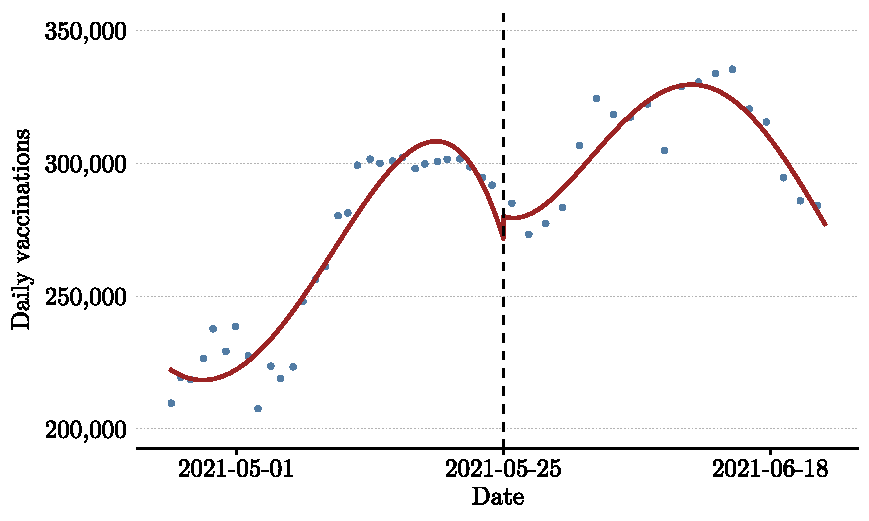
\includegraphics{bachelor_thesis_files/figure-latex/unnamed-chunk-2-1} \end{center}
\end{figure}

\noindent As other countries, Poland first dealt with a shortage of
vaccines, leading to necessary rationing, having to favor older and
chronically ill citizens first. Towards the summer, this shortage
significantly loosened its grip. Although the growth rate in the
vaccination rate increased significantly, for countries like Poland with
a comparably high vaccine hesitancy, the problem turned from a vaccine
shortage to a shortage of people willing to get vaccinated. Simply from
looking at figure 4.1, we can not observe a sharp or outstanding change
in the growth rate at the time of announcement or shortly
after\footnote{We would expect that the it takes several weeks for any significant change to be visible, since getting fully vaccinated takes/took around six to eight weeks}.
This is however also not expected, since the magnitude of the effect of
lotteries on vaccination rates is generally not very large, as outlined
in section 2.1.

\begin{figure}[h]
\caption{Vaccination rates (fully vaccinated) and the gap between Poland and synthetic Poland}

\begin{center}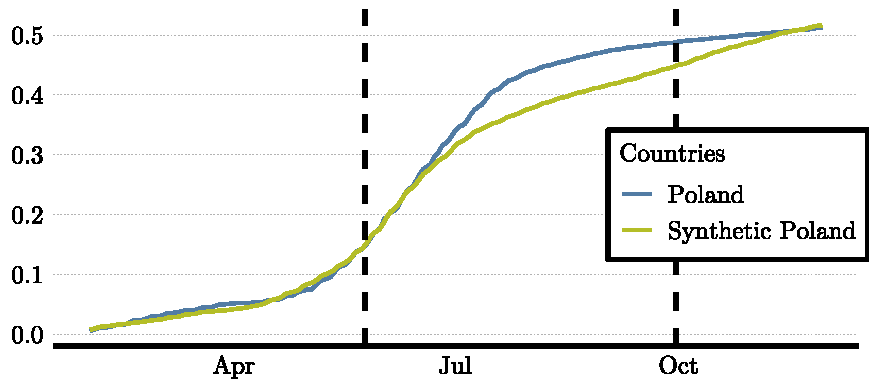
\includegraphics{bachelor_thesis_files/figure-latex/unnamed-chunk-3-1} \end{center}



\begin{center}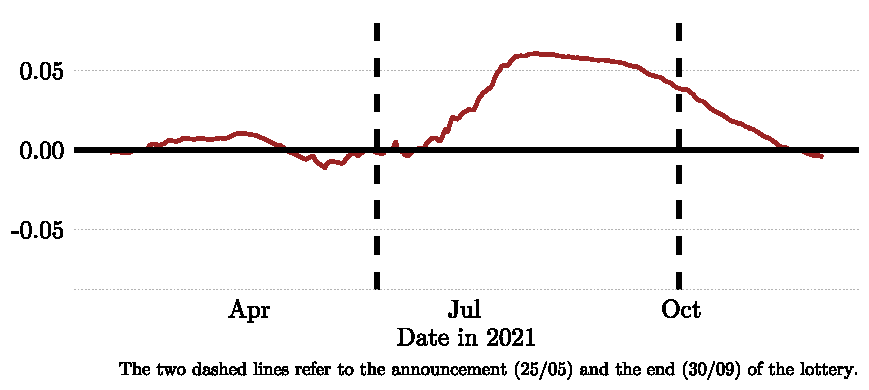
\includegraphics{bachelor_thesis_files/figure-latex/unnamed-chunk-3-2} \end{center}
\end{figure}

We therefore applied the synthetic control method, as described in
section 3.2. Figure 4.2 plots the vaccination rate (fully vaccinated)
for both Poland and synthetic Poland. We observe a solid, but not
perfect pre-treatment fit (too unspecific). From the intervention, we
can see a slow decoupling between Poland and its synthetic control. This
difference continues increase to around 5 percentage points. As time
progresses, the gap however tends to decrease again, and by the end of
November (after the end of the lottery), the vaccination rates of Poland
and synthetic Poland are back to the same level. Simply based on the
plot, one interpretation could be that the lottery successfully induces
some people who would have gotten vaccinated anyway to do this earlier,
to take advantage of the incentive provided by the government. It
however also suggests that the vaccine lottery was not particularly
effective in reaching new people. It has to be noted that the more time
has passed since the intervention, the synthetic control becomes more
unreliable, as the prediction intervals in figure \ldots{} show.
Therefore, the development in October and November should be interpreted
with caution, but at first glance, it seems like the lottery was not
successful in getting more people vaccinated, but only in getting people
vaccinated earlier.

Employing the permutation based inference techniques discussed in
section 4.1, also shows no signs of a significant effect. Figure
\ldots{} presents the placebo study. As can be seen, the magnitude of
the effect of Poland is not comparably high and does not stand out. This
finding also confirmed quantitatively. Using the discussed test
procedure, a p-value of around 0.5 is obtained. Therefore, the
hypothesis that the lottery had no effect in increasing vaccination
rates cannot be rejected, at any known/relevant significance level. The
findings of the permutation based inference are therefore in line with
the prediction intervals and do not suggest a statistically significant
effect of the lottery on vaccination rates (fully vaccinated).

\chapter{Discussion}

\chapter{Conclusion}


 
\backmatter
 
\renewcommand\refname{References}
\printbibliography[title=References]

\chapter{Appendix}
Hier steht ein Anhang.



\chapter{Affidavit}
\thispagestyle{empty}

% Dieser Text entspricht den genauen Vorgaben der Richtlinien für Bachelorarbeiten sowie der Prüfungsordnung (\§ 14a) 
% Stand: November 2014
I affirm that this Bachelor thesis was written by myself without any unauthorised third-party support. All used references and resources are clearly indicated. All quotes and citations are properly referenced. This thesis was never presented in the past in the same or similar form to any examination board. 

\noindent I agree that my thesis may be subject to electronic plagiarism check. For this purpose an anonymous copy may be distributed and uploaded to
servers within and outside the University of Mannheim.

\vspace{2\baselineskip}

\noindent German translation:\\
Ich versichere, dass ich die vorliegende Arbeit ohne Hilfe Dritter und ohne Benutzung anderer
als der angegebenen Quellen und Hilfsmittel angefertigt und die den benutzten Quellen
wörtlich oder inhaltlich entnommenen Stellen als solche kenntlich gemacht habe. Diese Arbeit
hat in gleicher oder ähnlicher Form noch keiner Prüfungsbehörde vorgelegen.

\noindent Ich bin damit einverstanden, dass meine Arbeit zum Zwecke eines Plagiatsabgleichs in
elektronischer Form anonymisiert versendet und gespeichert werden kann.

\vspace{4\baselineskip}
\begin{center}
\parbox{.8\textwidth}{Mannheim, 17/03/2023 \hfill Benedikt Stelter}
\end{center}


 
\end{document}
